% Created by tikzDevice version 0.10.1 on 2017-12-04 16:18:37
% !TEX encoding = UTF-8 Unicode
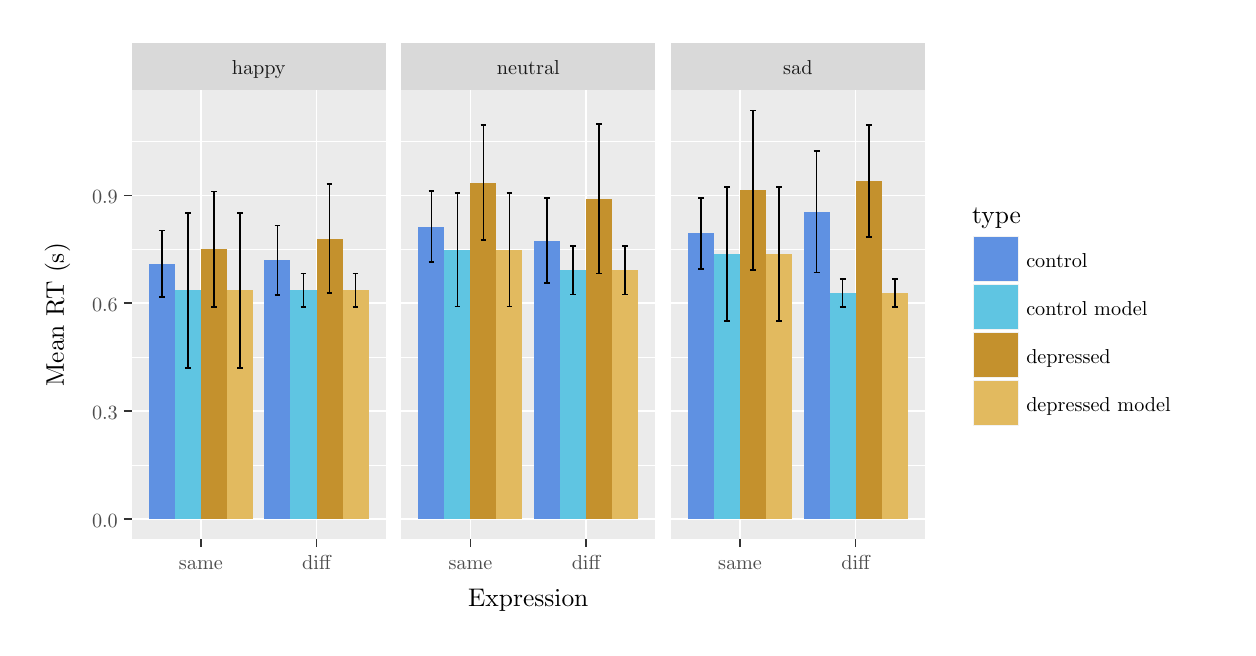
\begin{tikzpicture}[x=1pt,y=1pt]
\definecolor{fillColor}{RGB}{255,255,255}
\path[use as bounding box,fill=fillColor,fill opacity=0.00] (0,0) rectangle (433.62,216.81);
\begin{scope}
\path[clip] (  0.00,  0.00) rectangle (433.62,216.81);
\definecolor{drawColor}{RGB}{255,255,255}
\definecolor{fillColor}{RGB}{255,255,255}

\path[draw=drawColor,line width= 0.6pt,line join=round,line cap=round,fill=fillColor] ( -0.00,  0.00) rectangle (433.62,216.81);
\end{scope}
\begin{scope}
\path[clip] ( 37.53, 31.92) rectangle (129.44,194.25);
\definecolor{fillColor}{gray}{0.92}

\path[fill=fillColor] ( 37.53, 31.92) rectangle (129.44,194.25);
\definecolor{drawColor}{RGB}{255,255,255}

\path[draw=drawColor,line width= 0.3pt,line join=round] ( 37.53, 58.78) --
	(129.44, 58.78);

\path[draw=drawColor,line width= 0.3pt,line join=round] ( 37.53, 97.76) --
	(129.44, 97.76);

\path[draw=drawColor,line width= 0.3pt,line join=round] ( 37.53,136.73) --
	(129.44,136.73);

\path[draw=drawColor,line width= 0.3pt,line join=round] ( 37.53,175.70) --
	(129.44,175.70);

\path[draw=drawColor,line width= 0.6pt,line join=round] ( 37.53, 39.30) --
	(129.44, 39.30);

\path[draw=drawColor,line width= 0.6pt,line join=round] ( 37.53, 78.27) --
	(129.44, 78.27);

\path[draw=drawColor,line width= 0.6pt,line join=round] ( 37.53,117.24) --
	(129.44,117.24);

\path[draw=drawColor,line width= 0.6pt,line join=round] ( 37.53,156.21) --
	(129.44,156.21);

\path[draw=drawColor,line width= 0.6pt,line join=round] ( 62.60, 31.92) --
	( 62.60,194.25);

\path[draw=drawColor,line width= 0.6pt,line join=round] (104.37, 31.92) --
	(104.37,194.25);
\definecolor{fillColor}{RGB}{226,186,95}

\path[fill=fillColor] ( 72.00, 39.30) rectangle ( 81.40,121.94);
\definecolor{fillColor}{RGB}{196,145,45}

\path[fill=fillColor] ( 62.60, 39.30) rectangle ( 72.00,136.73);
\definecolor{fillColor}{RGB}{95,197,226}

\path[fill=fillColor] ( 53.20, 39.30) rectangle ( 62.60,121.94);
\definecolor{fillColor}{RGB}{95,145,226}

\path[fill=fillColor] ( 43.80, 39.30) rectangle ( 53.20,131.53);
\definecolor{fillColor}{RGB}{226,186,95}

\path[fill=fillColor] (113.77, 39.30) rectangle (123.17,121.87);
\definecolor{fillColor}{RGB}{196,145,45}

\path[fill=fillColor] (104.37, 39.30) rectangle (113.77,140.62);
\definecolor{fillColor}{RGB}{95,197,226}

\path[fill=fillColor] ( 94.97, 39.30) rectangle (104.37,121.87);
\definecolor{fillColor}{RGB}{95,145,226}

\path[fill=fillColor] ( 85.57, 39.30) rectangle ( 94.97,132.70);
\definecolor{drawColor}{RGB}{0,0,0}

\path[draw=drawColor,line width= 0.6pt,line join=round] ( 75.65,149.95) --
	( 77.74,149.95);

\path[draw=drawColor,line width= 0.6pt,line join=round] ( 76.70,149.95) --
	( 76.70, 93.93);

\path[draw=drawColor,line width= 0.6pt,line join=round] ( 75.65, 93.93) --
	( 77.74, 93.93);

\path[draw=drawColor,line width= 0.6pt,line join=round] ( 66.25,157.64) --
	( 68.34,157.64);

\path[draw=drawColor,line width= 0.6pt,line join=round] ( 67.30,157.64) --
	( 67.30,115.81);

\path[draw=drawColor,line width= 0.6pt,line join=round] ( 66.25,115.81) --
	( 68.34,115.81);

\path[draw=drawColor,line width= 0.6pt,line join=round] ( 56.85,149.95) --
	( 58.94,149.95);

\path[draw=drawColor,line width= 0.6pt,line join=round] ( 57.90,149.95) --
	( 57.90, 93.93);

\path[draw=drawColor,line width= 0.6pt,line join=round] ( 56.85, 93.93) --
	( 58.94, 93.93);

\path[draw=drawColor,line width= 0.6pt,line join=round] ( 47.45,143.48) --
	( 49.54,143.48);

\path[draw=drawColor,line width= 0.6pt,line join=round] ( 48.50,143.48) --
	( 48.50,119.58);

\path[draw=drawColor,line width= 0.6pt,line join=round] ( 47.45,119.58) --
	( 49.54,119.58);

\path[draw=drawColor,line width= 0.6pt,line join=round] (117.43,127.92) --
	(119.52,127.92);

\path[draw=drawColor,line width= 0.6pt,line join=round] (118.47,127.92) --
	(118.47,115.82);

\path[draw=drawColor,line width= 0.6pt,line join=round] (117.43,115.82) --
	(119.52,115.82);

\path[draw=drawColor,line width= 0.6pt,line join=round] (108.03,160.24) --
	(110.12,160.24);

\path[draw=drawColor,line width= 0.6pt,line join=round] (109.07,160.24) --
	(109.07,121.01);

\path[draw=drawColor,line width= 0.6pt,line join=round] (108.03,121.01) --
	(110.12,121.01);

\path[draw=drawColor,line width= 0.6pt,line join=round] ( 98.63,127.92) --
	(100.72,127.92);

\path[draw=drawColor,line width= 0.6pt,line join=round] ( 99.67,127.92) --
	( 99.67,115.82);

\path[draw=drawColor,line width= 0.6pt,line join=round] ( 98.63,115.82) --
	(100.72,115.82);

\path[draw=drawColor,line width= 0.6pt,line join=round] ( 89.23,145.30) --
	( 91.32,145.30);

\path[draw=drawColor,line width= 0.6pt,line join=round] ( 90.27,145.30) --
	( 90.27,120.10);

\path[draw=drawColor,line width= 0.6pt,line join=round] ( 89.23,120.10) --
	( 91.32,120.10);
\end{scope}
\begin{scope}
\path[clip] (134.94, 31.92) rectangle (226.85,194.25);
\definecolor{fillColor}{gray}{0.92}

\path[fill=fillColor] (134.94, 31.92) rectangle (226.85,194.25);
\definecolor{drawColor}{RGB}{255,255,255}

\path[draw=drawColor,line width= 0.3pt,line join=round] (134.94, 58.78) --
	(226.85, 58.78);

\path[draw=drawColor,line width= 0.3pt,line join=round] (134.94, 97.76) --
	(226.85, 97.76);

\path[draw=drawColor,line width= 0.3pt,line join=round] (134.94,136.73) --
	(226.85,136.73);

\path[draw=drawColor,line width= 0.3pt,line join=round] (134.94,175.70) --
	(226.85,175.70);

\path[draw=drawColor,line width= 0.6pt,line join=round] (134.94, 39.30) --
	(226.85, 39.30);

\path[draw=drawColor,line width= 0.6pt,line join=round] (134.94, 78.27) --
	(226.85, 78.27);

\path[draw=drawColor,line width= 0.6pt,line join=round] (134.94,117.24) --
	(226.85,117.24);

\path[draw=drawColor,line width= 0.6pt,line join=round] (134.94,156.21) --
	(226.85,156.21);

\path[draw=drawColor,line width= 0.6pt,line join=round] (160.00, 31.92) --
	(160.00,194.25);

\path[draw=drawColor,line width= 0.6pt,line join=round] (201.78, 31.92) --
	(201.78,194.25);
\definecolor{fillColor}{RGB}{226,186,95}

\path[fill=fillColor] (169.40, 39.30) rectangle (178.80,136.58);
\definecolor{fillColor}{RGB}{196,145,45}

\path[fill=fillColor] (160.00, 39.30) rectangle (169.40,160.76);
\definecolor{fillColor}{RGB}{95,197,226}

\path[fill=fillColor] (150.61, 39.30) rectangle (160.00,136.58);
\definecolor{fillColor}{RGB}{95,145,226}

\path[fill=fillColor] (141.21, 39.30) rectangle (150.61,144.91);
\definecolor{fillColor}{RGB}{226,186,95}

\path[fill=fillColor] (211.18, 39.30) rectangle (220.58,129.09);
\definecolor{fillColor}{RGB}{196,145,45}

\path[fill=fillColor] (201.78, 39.30) rectangle (211.18,155.04);
\definecolor{fillColor}{RGB}{95,197,226}

\path[fill=fillColor] (192.38, 39.30) rectangle (201.78,129.09);
\definecolor{fillColor}{RGB}{95,145,226}

\path[fill=fillColor] (182.98, 39.30) rectangle (192.38,139.85);
\definecolor{drawColor}{RGB}{0,0,0}

\path[draw=drawColor,line width= 0.6pt,line join=round] (173.06,157.15) --
	(175.15,157.15);

\path[draw=drawColor,line width= 0.6pt,line join=round] (174.10,157.15) --
	(174.10,116.02);

\path[draw=drawColor,line width= 0.6pt,line join=round] (173.06,116.02) --
	(175.15,116.02);

\path[draw=drawColor,line width= 0.6pt,line join=round] (163.66,181.54) --
	(165.75,181.54);

\path[draw=drawColor,line width= 0.6pt,line join=round] (164.70,181.54) --
	(164.70,139.97);

\path[draw=drawColor,line width= 0.6pt,line join=round] (163.66,139.97) --
	(165.75,139.97);

\path[draw=drawColor,line width= 0.6pt,line join=round] (154.26,157.15) --
	(156.35,157.15);

\path[draw=drawColor,line width= 0.6pt,line join=round] (155.31,157.15) --
	(155.31,116.02);

\path[draw=drawColor,line width= 0.6pt,line join=round] (154.26,116.02) --
	(156.35,116.02);

\path[draw=drawColor,line width= 0.6pt,line join=round] (144.86,157.77) --
	(146.95,157.77);

\path[draw=drawColor,line width= 0.6pt,line join=round] (145.91,157.77) --
	(145.91,132.05);

\path[draw=drawColor,line width= 0.6pt,line join=round] (144.86,132.05) --
	(146.95,132.05);

\path[draw=drawColor,line width= 0.6pt,line join=round] (214.84,137.83) --
	(216.92,137.83);

\path[draw=drawColor,line width= 0.6pt,line join=round] (215.88,137.83) --
	(215.88,120.35);

\path[draw=drawColor,line width= 0.6pt,line join=round] (214.84,120.35) --
	(216.92,120.35);

\path[draw=drawColor,line width= 0.6pt,line join=round] (205.44,182.06) --
	(207.52,182.06);

\path[draw=drawColor,line width= 0.6pt,line join=round] (206.48,182.06) --
	(206.48,128.02);

\path[draw=drawColor,line width= 0.6pt,line join=round] (205.44,128.02) --
	(207.52,128.02);

\path[draw=drawColor,line width= 0.6pt,line join=round] (196.04,137.83) --
	(198.13,137.83);

\path[draw=drawColor,line width= 0.6pt,line join=round] (197.08,137.83) --
	(197.08,120.35);

\path[draw=drawColor,line width= 0.6pt,line join=round] (196.04,120.35) --
	(198.13,120.35);

\path[draw=drawColor,line width= 0.6pt,line join=round] (186.64,155.17) --
	(188.73,155.17);

\path[draw=drawColor,line width= 0.6pt,line join=round] (187.68,155.17) --
	(187.68,124.52);

\path[draw=drawColor,line width= 0.6pt,line join=round] (186.64,124.52) --
	(188.73,124.52);
\end{scope}
\begin{scope}
\path[clip] (232.35, 31.92) rectangle (324.25,194.25);
\definecolor{fillColor}{gray}{0.92}

\path[fill=fillColor] (232.35, 31.92) rectangle (324.25,194.25);
\definecolor{drawColor}{RGB}{255,255,255}

\path[draw=drawColor,line width= 0.3pt,line join=round] (232.35, 58.78) --
	(324.25, 58.78);

\path[draw=drawColor,line width= 0.3pt,line join=round] (232.35, 97.76) --
	(324.25, 97.76);

\path[draw=drawColor,line width= 0.3pt,line join=round] (232.35,136.73) --
	(324.25,136.73);

\path[draw=drawColor,line width= 0.3pt,line join=round] (232.35,175.70) --
	(324.25,175.70);

\path[draw=drawColor,line width= 0.6pt,line join=round] (232.35, 39.30) --
	(324.25, 39.30);

\path[draw=drawColor,line width= 0.6pt,line join=round] (232.35, 78.27) --
	(324.25, 78.27);

\path[draw=drawColor,line width= 0.6pt,line join=round] (232.35,117.24) --
	(324.25,117.24);

\path[draw=drawColor,line width= 0.6pt,line join=round] (232.35,156.21) --
	(324.25,156.21);

\path[draw=drawColor,line width= 0.6pt,line join=round] (257.41, 31.92) --
	(257.41,194.25);

\path[draw=drawColor,line width= 0.6pt,line join=round] (299.19, 31.92) --
	(299.19,194.25);
\definecolor{fillColor}{RGB}{226,186,95}

\path[fill=fillColor] (266.81, 39.30) rectangle (276.21,135.12);
\definecolor{fillColor}{RGB}{196,145,45}

\path[fill=fillColor] (257.41, 39.30) rectangle (266.81,158.03);
\definecolor{fillColor}{RGB}{95,197,226}

\path[fill=fillColor] (248.01, 39.30) rectangle (257.41,135.12);
\definecolor{fillColor}{RGB}{95,145,226}

\path[fill=fillColor] (238.61, 39.30) rectangle (248.01,142.44);
\definecolor{fillColor}{RGB}{226,186,95}

\path[fill=fillColor] (308.59, 39.30) rectangle (317.99,120.96);
\definecolor{fillColor}{RGB}{196,145,45}

\path[fill=fillColor] (299.19, 39.30) rectangle (308.59,161.41);
\definecolor{fillColor}{RGB}{95,197,226}

\path[fill=fillColor] (289.79, 39.30) rectangle (299.19,120.96);
\definecolor{fillColor}{RGB}{95,145,226}

\path[fill=fillColor] (280.39, 39.30) rectangle (289.79,150.24);
\definecolor{drawColor}{RGB}{0,0,0}

\path[draw=drawColor,line width= 0.6pt,line join=round] (270.47,159.33) --
	(272.56,159.33);

\path[draw=drawColor,line width= 0.6pt,line join=round] (271.51,159.33) --
	(271.51,110.90);

\path[draw=drawColor,line width= 0.6pt,line join=round] (270.47,110.90) --
	(272.56,110.90);

\path[draw=drawColor,line width= 0.6pt,line join=round] (261.07,186.87) --
	(263.16,186.87);

\path[draw=drawColor,line width= 0.6pt,line join=round] (262.11,186.87) --
	(262.11,129.19);

\path[draw=drawColor,line width= 0.6pt,line join=round] (261.07,129.19) --
	(263.16,129.19);

\path[draw=drawColor,line width= 0.6pt,line join=round] (251.67,159.33) --
	(253.76,159.33);

\path[draw=drawColor,line width= 0.6pt,line join=round] (252.71,159.33) --
	(252.71,110.90);

\path[draw=drawColor,line width= 0.6pt,line join=round] (251.67,110.90) --
	(253.76,110.90);

\path[draw=drawColor,line width= 0.6pt,line join=round] (242.27,155.17) --
	(244.36,155.17);

\path[draw=drawColor,line width= 0.6pt,line join=round] (243.31,155.17) --
	(243.31,129.71);

\path[draw=drawColor,line width= 0.6pt,line join=round] (242.27,129.71) --
	(244.36,129.71);

\path[draw=drawColor,line width= 0.6pt,line join=round] (312.24,125.94) --
	(314.33,125.94);

\path[draw=drawColor,line width= 0.6pt,line join=round] (313.29,125.94) --
	(313.29,115.98);

\path[draw=drawColor,line width= 0.6pt,line join=round] (312.24,115.98) --
	(314.33,115.98);

\path[draw=drawColor,line width= 0.6pt,line join=round] (302.84,181.54) --
	(304.93,181.54);

\path[draw=drawColor,line width= 0.6pt,line join=round] (303.89,181.54) --
	(303.89,141.27);

\path[draw=drawColor,line width= 0.6pt,line join=round] (302.84,141.27) --
	(304.93,141.27);

\path[draw=drawColor,line width= 0.6pt,line join=round] (293.44,125.94) --
	(295.53,125.94);

\path[draw=drawColor,line width= 0.6pt,line join=round] (294.49,125.94) --
	(294.49,115.98);

\path[draw=drawColor,line width= 0.6pt,line join=round] (293.44,115.98) --
	(295.53,115.98);

\path[draw=drawColor,line width= 0.6pt,line join=round] (284.04,172.19) --
	(286.13,172.19);

\path[draw=drawColor,line width= 0.6pt,line join=round] (285.09,172.19) --
	(285.09,128.28);

\path[draw=drawColor,line width= 0.6pt,line join=round] (284.04,128.28) --
	(286.13,128.28);
\end{scope}
\begin{scope}
\path[clip] ( 37.53,194.25) rectangle (129.44,211.31);
\definecolor{fillColor}{gray}{0.85}

\path[fill=fillColor] ( 37.53,194.25) rectangle (129.44,211.31);
\definecolor{drawColor}{gray}{0.10}

\node[text=drawColor,anchor=base,inner sep=0pt, outer sep=0pt, scale=  0.73] at ( 83.49,199.75) {happy};
\end{scope}
\begin{scope}
\path[clip] (134.94,194.25) rectangle (226.85,211.31);
\definecolor{fillColor}{gray}{0.85}

\path[fill=fillColor] (134.94,194.25) rectangle (226.85,211.31);
\definecolor{drawColor}{gray}{0.10}

\node[text=drawColor,anchor=base,inner sep=0pt, outer sep=0pt, scale=  0.73] at (180.89,199.75) {neutral};
\end{scope}
\begin{scope}
\path[clip] (232.35,194.25) rectangle (324.25,211.31);
\definecolor{fillColor}{gray}{0.85}

\path[fill=fillColor] (232.35,194.25) rectangle (324.25,211.31);
\definecolor{drawColor}{gray}{0.10}

\node[text=drawColor,anchor=base,inner sep=0pt, outer sep=0pt, scale=  0.73] at (278.30,199.75) {sad};
\end{scope}
\begin{scope}
\path[clip] (  0.00,  0.00) rectangle (433.62,216.81);
\definecolor{drawColor}{gray}{0.20}

\path[draw=drawColor,line width= 0.6pt,line join=round] ( 62.60, 29.17) --
	( 62.60, 31.92);

\path[draw=drawColor,line width= 0.6pt,line join=round] (104.37, 29.17) --
	(104.37, 31.92);
\end{scope}
\begin{scope}
\path[clip] (  0.00,  0.00) rectangle (433.62,216.81);
\definecolor{drawColor}{gray}{0.30}

\node[text=drawColor,anchor=base,inner sep=0pt, outer sep=0pt, scale=  0.73] at ( 62.60, 20.91) {same};

\node[text=drawColor,anchor=base,inner sep=0pt, outer sep=0pt, scale=  0.73] at (104.37, 20.91) {diff};
\end{scope}
\begin{scope}
\path[clip] (  0.00,  0.00) rectangle (433.62,216.81);
\definecolor{drawColor}{gray}{0.20}

\path[draw=drawColor,line width= 0.6pt,line join=round] (160.00, 29.17) --
	(160.00, 31.92);

\path[draw=drawColor,line width= 0.6pt,line join=round] (201.78, 29.17) --
	(201.78, 31.92);
\end{scope}
\begin{scope}
\path[clip] (  0.00,  0.00) rectangle (433.62,216.81);
\definecolor{drawColor}{gray}{0.30}

\node[text=drawColor,anchor=base,inner sep=0pt, outer sep=0pt, scale=  0.73] at (160.00, 20.91) {same};

\node[text=drawColor,anchor=base,inner sep=0pt, outer sep=0pt, scale=  0.73] at (201.78, 20.91) {diff};
\end{scope}
\begin{scope}
\path[clip] (  0.00,  0.00) rectangle (433.62,216.81);
\definecolor{drawColor}{gray}{0.20}

\path[draw=drawColor,line width= 0.6pt,line join=round] (257.41, 29.17) --
	(257.41, 31.92);

\path[draw=drawColor,line width= 0.6pt,line join=round] (299.19, 29.17) --
	(299.19, 31.92);
\end{scope}
\begin{scope}
\path[clip] (  0.00,  0.00) rectangle (433.62,216.81);
\definecolor{drawColor}{gray}{0.30}

\node[text=drawColor,anchor=base,inner sep=0pt, outer sep=0pt, scale=  0.73] at (257.41, 20.91) {same};

\node[text=drawColor,anchor=base,inner sep=0pt, outer sep=0pt, scale=  0.73] at (299.19, 20.91) {diff};
\end{scope}
\begin{scope}
\path[clip] (  0.00,  0.00) rectangle (433.62,216.81);
\definecolor{drawColor}{gray}{0.30}

\node[text=drawColor,anchor=base east,inner sep=0pt, outer sep=0pt, scale=  0.73] at ( 32.58, 36.27) {0.0};

\node[text=drawColor,anchor=base east,inner sep=0pt, outer sep=0pt, scale=  0.73] at ( 32.58, 75.24) {0.3};

\node[text=drawColor,anchor=base east,inner sep=0pt, outer sep=0pt, scale=  0.73] at ( 32.58,114.21) {0.6};

\node[text=drawColor,anchor=base east,inner sep=0pt, outer sep=0pt, scale=  0.73] at ( 32.58,153.18) {0.9};
\end{scope}
\begin{scope}
\path[clip] (  0.00,  0.00) rectangle (433.62,216.81);
\definecolor{drawColor}{gray}{0.20}

\path[draw=drawColor,line width= 0.6pt,line join=round] ( 34.78, 39.30) --
	( 37.53, 39.30);

\path[draw=drawColor,line width= 0.6pt,line join=round] ( 34.78, 78.27) --
	( 37.53, 78.27);

\path[draw=drawColor,line width= 0.6pt,line join=round] ( 34.78,117.24) --
	( 37.53,117.24);

\path[draw=drawColor,line width= 0.6pt,line join=round] ( 34.78,156.21) --
	( 37.53,156.21);
\end{scope}
\begin{scope}
\path[clip] (  0.00,  0.00) rectangle (433.62,216.81);
\definecolor{drawColor}{RGB}{0,0,0}

\node[text=drawColor,anchor=base,inner sep=0pt, outer sep=0pt, scale=  0.92] at (180.89,  7.83) {Expression};
\end{scope}
\begin{scope}
\path[clip] (  0.00,  0.00) rectangle (433.62,216.81);
\definecolor{drawColor}{RGB}{0,0,0}

\node[text=drawColor,rotate= 90.00,anchor=base,inner sep=0pt, outer sep=0pt, scale=  0.92] at ( 13.08,113.08) {Mean RT (s)};
\end{scope}
\begin{scope}
\path[clip] (  0.00,  0.00) rectangle (433.62,216.81);
\definecolor{fillColor}{RGB}{255,255,255}

\path[fill=fillColor] (335.63, 66.75) rectangle (428.12,159.42);
\end{scope}
\begin{scope}
\path[clip] (  0.00,  0.00) rectangle (433.62,216.81);
\definecolor{drawColor}{RGB}{0,0,0}

\node[text=drawColor,anchor=base west,inner sep=0pt, outer sep=0pt, scale=  0.92] at (341.32,146.15) {type};
\end{scope}
\begin{scope}
\path[clip] (  0.00,  0.00) rectangle (433.62,216.81);
\definecolor{drawColor}{RGB}{255,255,255}
\definecolor{fillColor}{gray}{0.95}

\path[draw=drawColor,line width= 0.6pt,line join=round,line cap=round,fill=fillColor] (341.32,124.47) rectangle (358.67,141.82);
\end{scope}
\begin{scope}
\path[clip] (  0.00,  0.00) rectangle (433.62,216.81);
\definecolor{fillColor}{RGB}{95,145,226}

\path[fill=fillColor] (342.04,125.18) rectangle (357.96,141.11);
\end{scope}
\begin{scope}
\path[clip] (  0.00,  0.00) rectangle (433.62,216.81);
\definecolor{drawColor}{RGB}{255,255,255}
\definecolor{fillColor}{gray}{0.95}

\path[draw=drawColor,line width= 0.6pt,line join=round,line cap=round,fill=fillColor] (341.32,107.13) rectangle (358.67,124.47);
\end{scope}
\begin{scope}
\path[clip] (  0.00,  0.00) rectangle (433.62,216.81);
\definecolor{fillColor}{RGB}{95,197,226}

\path[fill=fillColor] (342.04,107.84) rectangle (357.96,123.76);
\end{scope}
\begin{scope}
\path[clip] (  0.00,  0.00) rectangle (433.62,216.81);
\definecolor{drawColor}{RGB}{255,255,255}
\definecolor{fillColor}{gray}{0.95}

\path[draw=drawColor,line width= 0.6pt,line join=round,line cap=round,fill=fillColor] (341.32, 89.78) rectangle (358.67,107.13);
\end{scope}
\begin{scope}
\path[clip] (  0.00,  0.00) rectangle (433.62,216.81);
\definecolor{fillColor}{RGB}{196,145,45}

\path[fill=fillColor] (342.04, 90.49) rectangle (357.96,106.42);
\end{scope}
\begin{scope}
\path[clip] (  0.00,  0.00) rectangle (433.62,216.81);
\definecolor{drawColor}{RGB}{255,255,255}
\definecolor{fillColor}{gray}{0.95}

\path[draw=drawColor,line width= 0.6pt,line join=round,line cap=round,fill=fillColor] (341.32, 72.44) rectangle (358.67, 89.78);
\end{scope}
\begin{scope}
\path[clip] (  0.00,  0.00) rectangle (433.62,216.81);
\definecolor{fillColor}{RGB}{226,186,95}

\path[fill=fillColor] (342.04, 73.15) rectangle (357.96, 89.07);
\end{scope}
\begin{scope}
\path[clip] (  0.00,  0.00) rectangle (433.62,216.81);
\definecolor{drawColor}{RGB}{0,0,0}

\node[text=drawColor,anchor=base west,inner sep=0pt, outer sep=0pt, scale=  0.73] at (360.84,130.12) {control};
\end{scope}
\begin{scope}
\path[clip] (  0.00,  0.00) rectangle (433.62,216.81);
\definecolor{drawColor}{RGB}{0,0,0}

\node[text=drawColor,anchor=base west,inner sep=0pt, outer sep=0pt, scale=  0.73] at (360.84,112.77) {control model};
\end{scope}
\begin{scope}
\path[clip] (  0.00,  0.00) rectangle (433.62,216.81);
\definecolor{drawColor}{RGB}{0,0,0}

\node[text=drawColor,anchor=base west,inner sep=0pt, outer sep=0pt, scale=  0.73] at (360.84, 95.43) {depressed};
\end{scope}
\begin{scope}
\path[clip] (  0.00,  0.00) rectangle (433.62,216.81);
\definecolor{drawColor}{RGB}{0,0,0}

\node[text=drawColor,anchor=base west,inner sep=0pt, outer sep=0pt, scale=  0.73] at (360.84, 78.08) {depressed model};
\end{scope}
\end{tikzpicture}
